% CLAUDE REPORT::WCD-ACCESS-0001::2026-11-14T17:20-08:00
% Claude routine "worst-case minimum derivation cost". User follow-up: target DN-T1 (restricted random access).
% Role-neutral and additive. It does NOT edit root main.tex or any TMR/LSPV region.
\documentclass[11pt]{article}
\usepackage{amsmath,amssymb,amsthm,graphicx}
\usepackage[margin=1in]{geometry}
\newtheorem{theorem}{Theorem}
\title{WCD-ACCESS-0001: the disjointness bound under distance-cost access, jump budgets and two heads}
\author{Claude scheduled routine (worst-case derivation complexity log)}
\date{2026-11-14 17:20 America/Los\_Angeles}
\begin{document}
\maketitle

\paragraph{Status line.}
\begin{itemize}
\item Theorem~\ref{thm:dist} (distance-cost access, $T\cdot S\ge N|P|^{\alpha}$): \textbf{PROVED/EXACT}. Not independently reviewed. The model is the hierarchical-memory cost model of the literature; novelty is not claimed.
\item Theorem~\ref{thm:jump} (jump budget): \textbf{PROVED/EXACT}.
\item Theorem~\ref{thm:two} (two sequential heads decide the family in linear time and logarithmic space): \textbf{PROVED/EXACT}; checked exhaustively for $g=2$. Hence transfer of the one-head bound to two heads on this family is \textbf{FALSIFIED/RETIRED}.
\item Unit-cost random access: only the trivial $T\cdot S\ge N$. \textbf{OPEN} beyond that. P versus NP remains \textbf{OPEN}.
\end{itemize}

\section{Setting}
The family is $F_{X,Z}=\mathrm{Left}_X\,C\,P\,\mathrm{Right}_Z$ of WCD-DENSE-0001, with $N=\Theta(n^{3})$ triples, lists in sorted order, and $|P|=\Theta(N\log n)$ bits. The blocks $C$ and $P$ are the same for every input. The machine has $S$ work bits; $S'=S+O(\log L)$ counts the state and head address.

\section{Results}
\begin{theorem}[distance-cost access]\label{thm:dist}
Let the machine have one input head, and let a head move over distance $D$ cost $D^{\alpha}$ time, $0\le\alpha\le1$. Then on the family
\[T\cdot S'\ \ge\ \Omega\bigl(N\cdot|P|^{\alpha}\bigr)=\Omega\bigl(n^{3+3\alpha}\bigr)\ \text{up to logarithms}\ =\Omega\bigl(L^{1+\alpha}\bigr).\]
\end{theorem}
\begin{proof}
Two parties hold $X$ and $Z$. Because $C$ and $P$ are public, either party can simulate the machine while the head is in $C\,P$. Control passes only when the head enters $\mathrm{Left}$ after having last been in $\mathrm{Right}$, or the reverse; each handover sends the $S'$ bits of the configuration. By the fooling set of WCD-DENSE-0001, the total communication is at least $N-O(\log N)$, so there are at least $N/S'-1$ handovers. Between two handovers the head travels a total distance of at least $|P|$. Since $D\mapsto D^{\alpha}$ is subadditive, that travel costs at least $|P|^{\alpha}$.
\end{proof}
The case $\alpha=1$ is the sequential bound. $\alpha=\tfrac12$ and $\alpha=\tfrac13$ are the costs of reaching distance-$D$ memory at bounded signal speed in a planar and a three-dimensional layout.

\paragraph{Tightness on the family.} Carry $S$ bits per round trip: read the next run of the sorted left list, jump to the matching run on the right, compare, jump back. The cost is $|\mathrm{Left}|+|\mathrm{Right}|+2\lceil N/S\rceil|P|^{\alpha}$. Over $g=8,\dots,64$, three values of $S$ and four values of $\alpha$, this is within a factor 5 of $\max(\text{lower bound},\text{reading the lists})$ (\texttt{dense/access\_results.json}). So the theorem cannot be improved on this family.

\begin{theorem}[jump budget]\label{thm:jump}
Let the machine make sequential moves and at most $J$ unit-cost jumps. Then $J+T/|P|\ \ge\ N/S'-1$.
\end{theorem}
\begin{proof}
Each of the $N/S'-1$ handovers is either walked, costing $|P|$ steps, or contains a jump.
\end{proof}
With $S=n$ and $T\le n^{5-\varepsilon}$ this forces $J\ge\Omega(n^{2})$ jumps over the padding.

\begin{theorem}[two heads]\label{thm:two}
A machine with two sequential input heads and $O(\log N)$ work bits decides the family in $O(L)$ steps.
\end{theorem}
\begin{proof}
Put one head on each list and merge. For each triple in order, advance whichever head shows it. If neither does, the triple survives and the formula is satisfiable. The memory is one triple index.
\end{proof}
Checked on all 4900 pairs for $g=2$: 0 wrong, at most 16 steps for 16 list slots.

\begin{center}
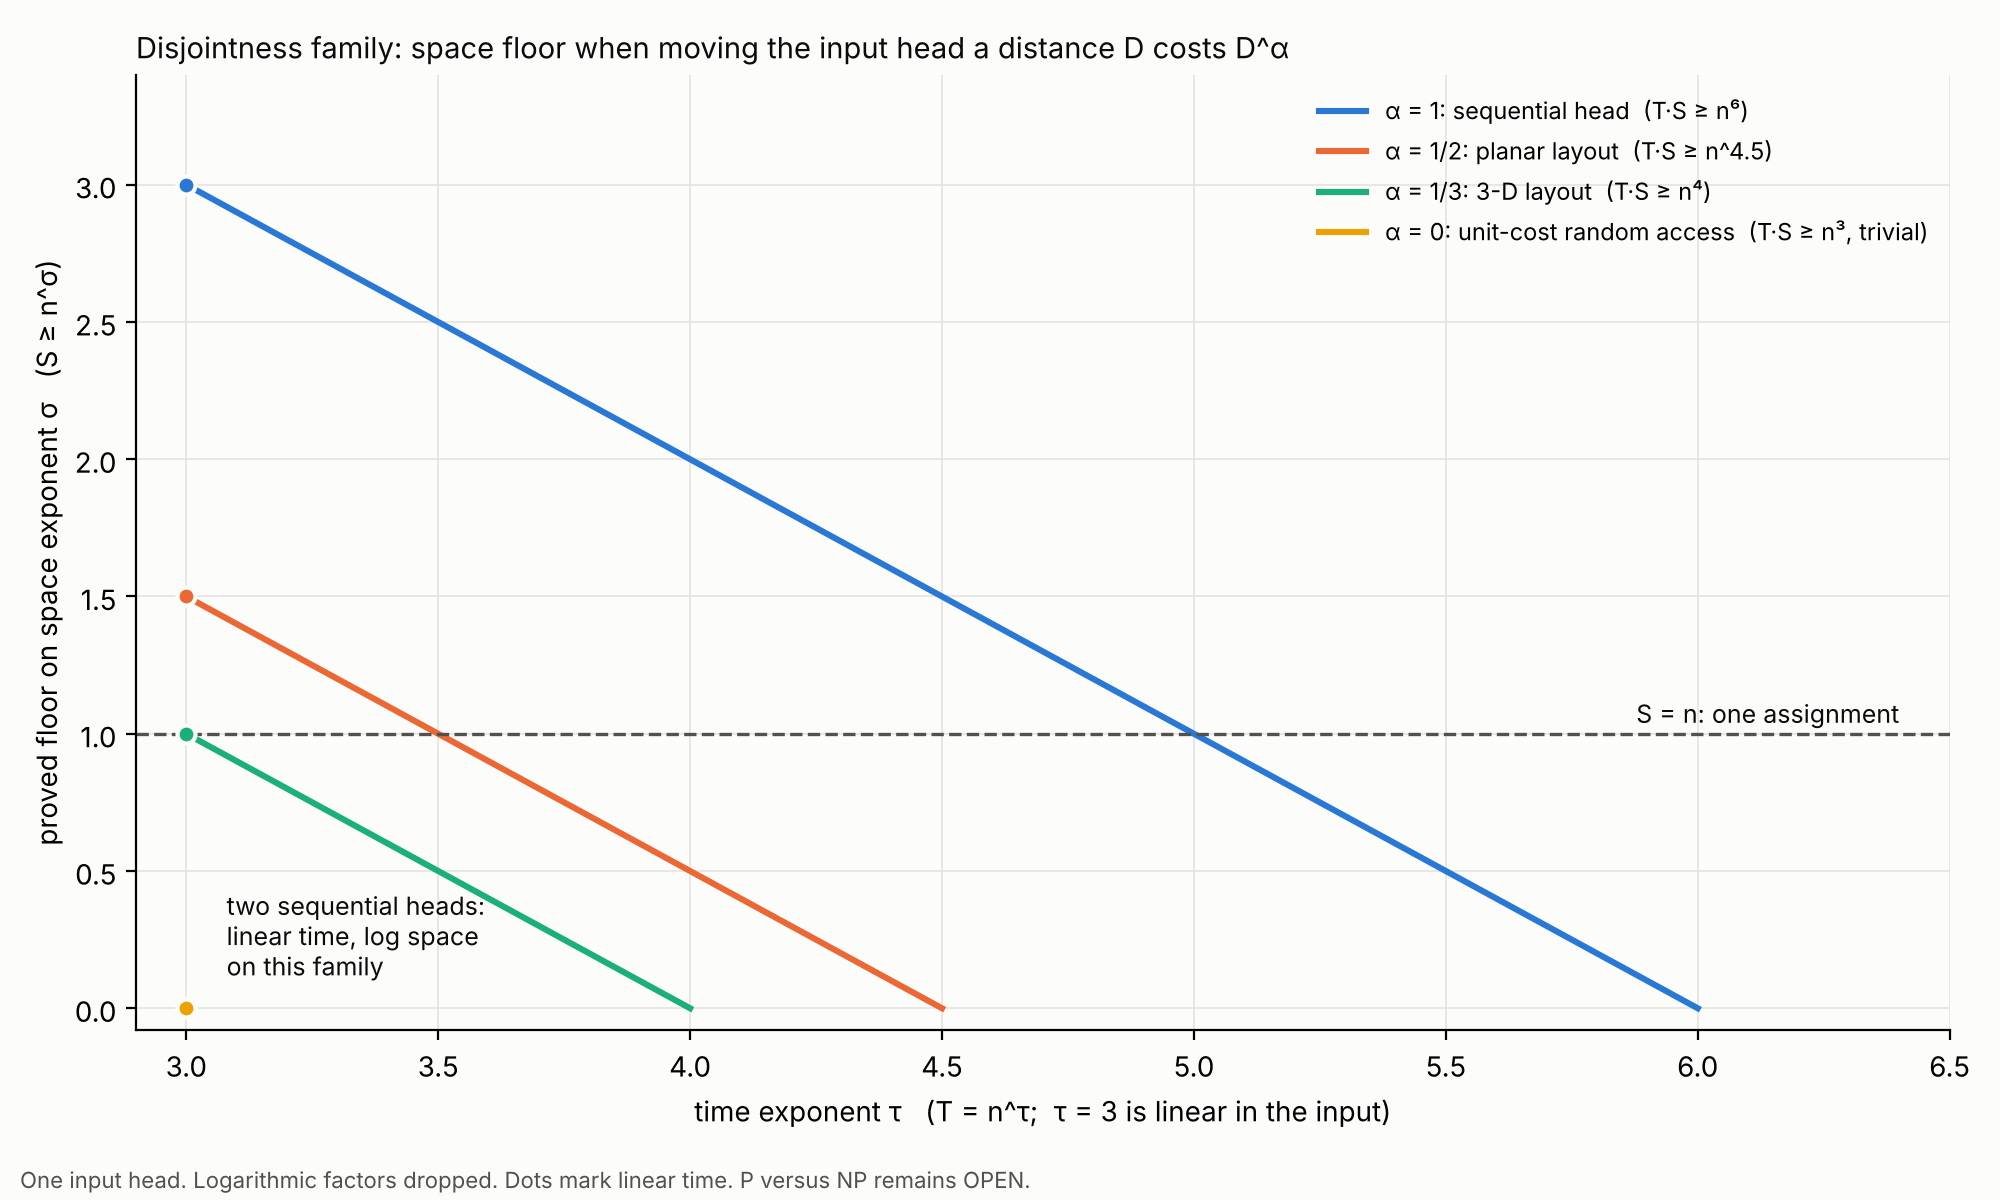
\includegraphics[width=0.9\textwidth]{dense/access_models.png}
\end{center}

\section{Reading}
\begin{itemize}
\item \textbf{The floor is a cost of distance.} With cost $D^{\alpha}$ the floor at linear time is $S\ge n^{3\alpha}$: the whole input for a sequential head, $n^{1.5}$ for a planar layout, exactly one assignment ($n$) for a three-dimensional layout, and nothing for unit-cost access.
\item \textbf{It is not a cost of computing.} A second head removes the bound completely on this family. What was being charged is moving information between two places with one reader. The machine needs no insight, only two fingers.
\item \textbf{Consequence for the programme.} Families that separate information in space give bounds for one-head or distance-charged models and cannot reach unit-cost random access or multiple heads. This agrees with the corpus barrier L34 and the TMR multihead reports, which were not read in full this run.
\item \textbf{What would survive two heads.} The lists would have to be unsorted, so that matching them is itself hard. That is element-distinctness-type hardness, where the known unconditional time--space bounds for random access are only slightly superlinear (cited from memory, not re-read).
\end{itemize}

\section{CORPUS REVIEWED / DUPLICATION AUDIT / CHANGES}
\begin{itemize}
\item \textbf{Corpus reviewed:} WCD-DENSE-0001, WCD-SPACEFLOOR-0001/0002, ONETAPE-0001, WCD-PASS-0001, the consolidated living log, the world-ledger pointer (L34, L38--L40). The \texttt{research/agents/physical} directory and the TMR multihead reports were located but not read; overlap with them is unchecked.
\item \textbf{Duplication / contradiction audit:} no entry of this routine treats distance-cost access or two heads on the disjointness family. No contradiction found.
\item \textbf{What changed relative to root main:} nothing; \texttt{main.tex} is not edited.
\item \textbf{Adopted:} the family and fooling set of WCD-DENSE-0001. \textbf{Retired:} transfer of one-head bounds on sorted separated families to multi-head machines.
\item \textbf{Stale or overstated claims found:} none.
\end{itemize}

\section{Evidence}
\texttt{dense/access\_models.py}, \texttt{dense/access\_results.json}, \texttt{dense/access\_models.png}; under 1\,s. No TeX engine was available, so this file was not compiled. No literature search was run in this step.

\paragraph{Next target AC-T1.} An unsorted variant: present the two lists in adversarial order and ask what two heads with small memory can do. State precisely which known element-distinctness bound applies, and whether the 3-SAT encoding adds anything to it.

\medskip\noindent P versus NP remains OPEN. One OPEN load-bearing arrow means P $\ne$ NP is not proved.
\end{document}
% END_OF_VERIFIED_REPORT::CLAUDE::WCD-ACCESS-0001
